The basic clustering algorithm, called \idbscan and described in
details in Ref.~\cite{iDBSCAN}, represents an improvement of the
neighboring pixels clusters, called \nnc, previously used to study the
performance of the \lemon detector with \fe radioactive
source~\cite{bib:fe55}. It is briefly described also here, since it
represents the seeding for the final clustering algorithm.

The energy deposition in the sensitive volume of the TPC is estimated
from the two-dimensional (2D) projection on the $x$--$y$ axes of the
light emitted in the multiplication process within the GEMs
planes. The pattern shows a large variation, depending on the
interacting particle. For images recorded with the \fe calibration
source, the signature of the typical 5.9\keV photons is a spot of few
mm$^2$, with the exact size depending on the diffusion in the
gas, \ie, on the distance from the anode, along $z$, of the point
where the energy release happens (see Fig.~\ref{fig:signals}
left). Muons from cosmic rays travel across the gas volume and leave a
typical signature of a straight track, shown in
Fig.~\ref{fig:typicalimage1} (right), but with several agglomeration
with larger density along the path. Natural radioactivity shows an
irregular pattern, sometimes curly, with several kinks along the
path. Finally, the signal from nuclear recoils due to neutrons,
originated by the \ambe source, is expected to be spot-like, or to
emerge as short straight tracks with a length smaller than 1\unit{mm}
for energies below 100\keV, as shown by Fig.~\ref{fig:range}.

Their track length and their size is found to depend a lot on the
initial energy of the impinging neutron, and also on the mass of the
recoiling nucleus in the He-CF$_4$ gas mixture utilized in
the \lemon detector.

Thus, the clustering algorithm needs to be flexible enough to
efficiently reconstruct a diverse set of patterns, from small round
spots to long and kinky tracks. A first step of the clustering,
called \textit{seeding}, is used: it focuses in the clustering of
spot-like neighboring pixels.  The method applied for the \lemon
detector is an evolution of the classic \dbscan
algorithm~\cite{dbscan}.  This is a non-parametric, density-based
clustering, which groups together pixels above threshold with many
neighbors, within a circle with a radius $\epsilon$. Its distinctive
characteristics making this method very suitable to the \lemon case is
its ability to label as outliers, and so not to include in the
clusters, pixels that lie isolated in low-density regions, \ie, pixels
from electronic noise of the sensor surviving the zero
suppression. The extension of \dbscan used for \lemon data analysis
consists in including a third dimension to the phase space of the
points considered, adding to the pixel position ($x$--$y$ coordinates)
the measured number of photons in that pixel, $N_{ph}$.  This approach
improves the combinatorial background rejection and the energy
resolution with respect the previously used \nnc algorithm, as
described in details in Ref.~\cite{iDBSCAN}.

To be as inclusive as possible, and since different interactions may
have vastly different intensities, even varying along the track, the
clustering procedure is iterated three times.  First, the \dbscan
parameters were tuned to form clusters of dense (in $x$--$y$ dimension)
and intense (in the $N_{ph}$ dimension) pixels. The density in 3D is
called \textit{sparsity}.  This step typically identifies either rare
hot spots of the GEMs, or, efficiently, short nuclear recoils. The
pixels belonging to the reconstructed clusters are then removed from
the image, and the \dbscan procedure is repeated, with looser sparsity
parameters. The second iteration is tuned to efficiently reconstruct
\fe round spots and slices of tracks from nuclear recoils with lower
intensity. It also collects the agglomeration with larger density
along cosmic tracks, clearly visible in the example in
Fig.~\ref{fig:typicalimage1} (right).  A third iteration of \dbscan
with even looser parameters is finally executed, targeting faint
portions of a cluster. These are especially used as a proxy for the
characterization of clustered noisy pixels, while the first two are
used as seeds for the final clustering step, described in
Sec.~\ref{sec:supercl}.

To be computationally viable, the \idbscan basic clustering is
performed on the image with reduced resolution, 512$\times$512. In
typical images this allows the basic cluster reconstruction to be run
in approximately 1\unit{s} on an \texttt{Intel Xeon
E5-2620}~2.00\unit{GHz} and 64\unit{GB} RAM. The reconstruction
algorithm is implemented in \PYTHONthree~\cite{python3}, and
interfaced with CERN \ROOT v6~\cite{root}.


Examples of clustered pixels in two cases are shown in
Fig.~\ref{fig:basic_clusters}. The left panel shows an example of
clusters reconstructed on the low-resolution image of one event
with \fe source. Three spots are clearly visible: one, as typical for
events with this calibration source with a moderate activity, is
reconstructed by a single cluster of the second iteration. The other
two are close enough that are merged in a single cluster of the same
iteration. The cases of merged spots containing twice the energy of a
single X-ray deposit, given the activity of the \fe source, represent
about one tenth of the clusters in this set of runs. The energy
resolution is good enough to distinguish statistically the single and
merged spots, as will be described in Sec.~\ref{sec:calibration}.  The
optimization of the \idbscan parameters is done assuming a low pileup
of events, typical of the running conditions for a future underground
run of the \cygno project, of which \lemon is the prototype, where the
occurrences of such cases are expected to be negligible.

The right panel shows the outcome of the \idbscan algorithm on a
longer track, presumably from natural radioactivity, and one possible
short nuclear recoil.  The nuclear recoil candidate is very dense,
highly-energetic, and isolated. Therefore, it is reconstructed as a
single cluster in the first iteration. The long track shows several
clusters with higher intensity. One of them has a large energy, and it
is reconstructed as an isolated single iteration-1 cluster. The rest
of the track is reconstructed by multiple iteration-2 clusters, which
are split where the energy deposition has a minimum extending across
too many pixels to be joined together in the same cluster. Events like
these, which are frequent for muons, natural radioactivity, but also
signals from $\alpha$-particles with higher energy, originating by the
possible interaction of neutrons with the plastic material of the
field cage, justify the need of the subsequent step of
the \textit{superclustering}, which follows the track without
splitting it in parts. This is described in the following section.
%
\begin{figure}[ht]
  \begin{center}
     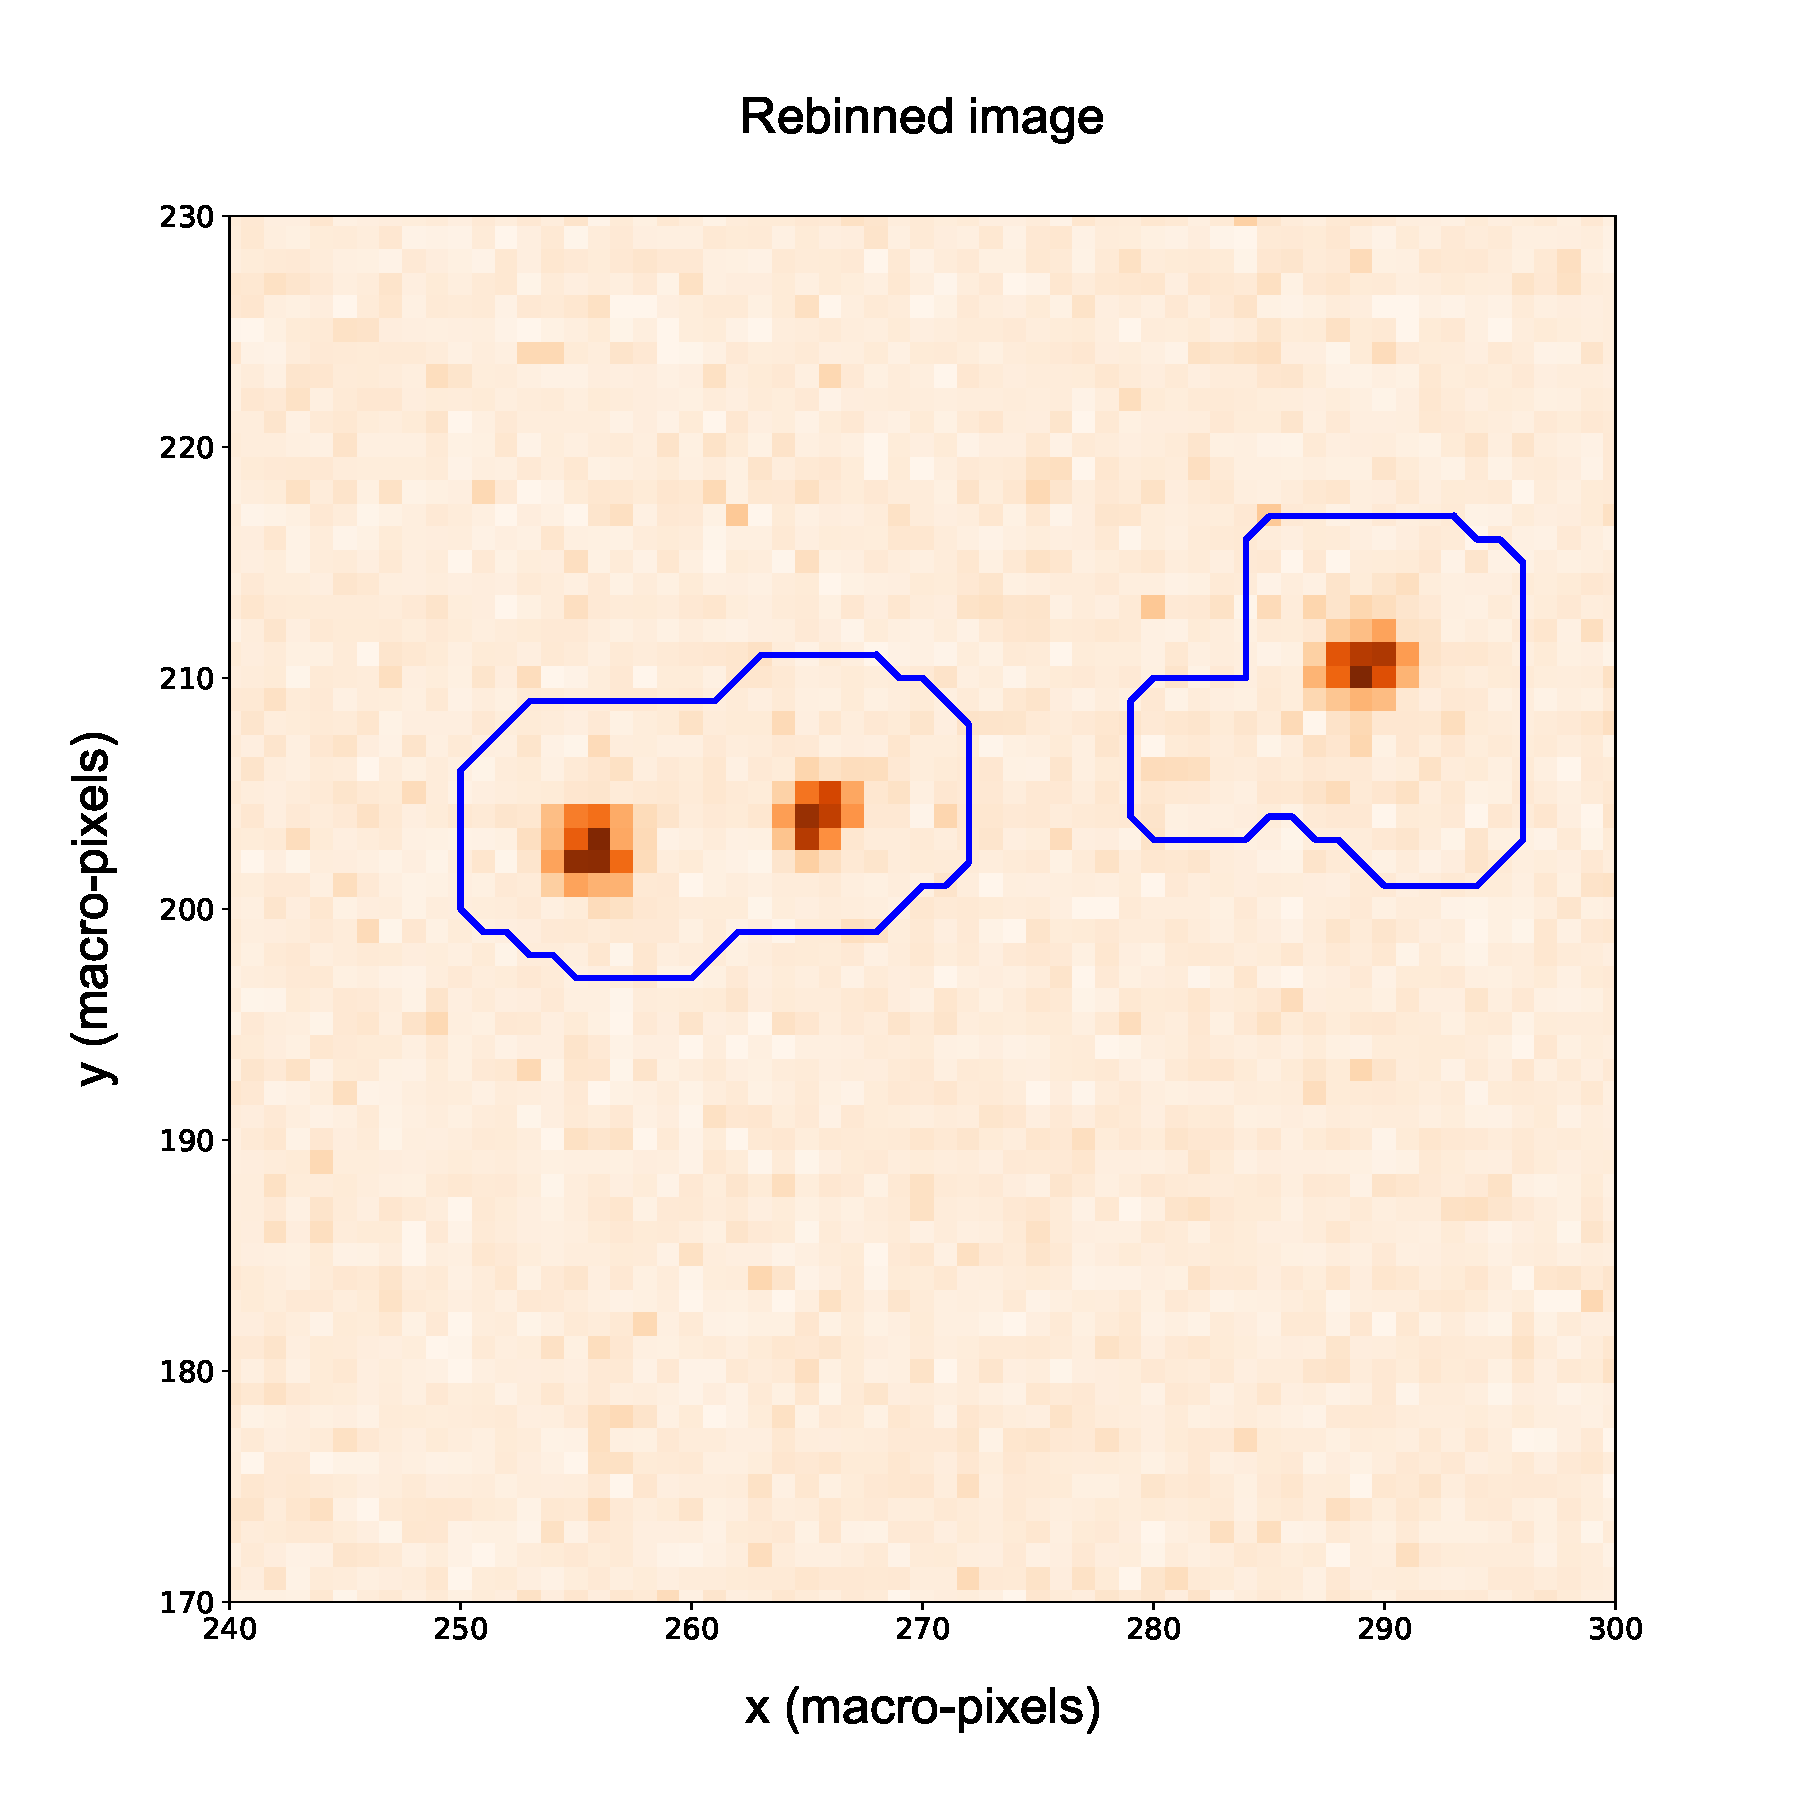
\includegraphics[width=0.49\linewidth]{figures/pic_run01843_ev93_2nd_3D_paper}
      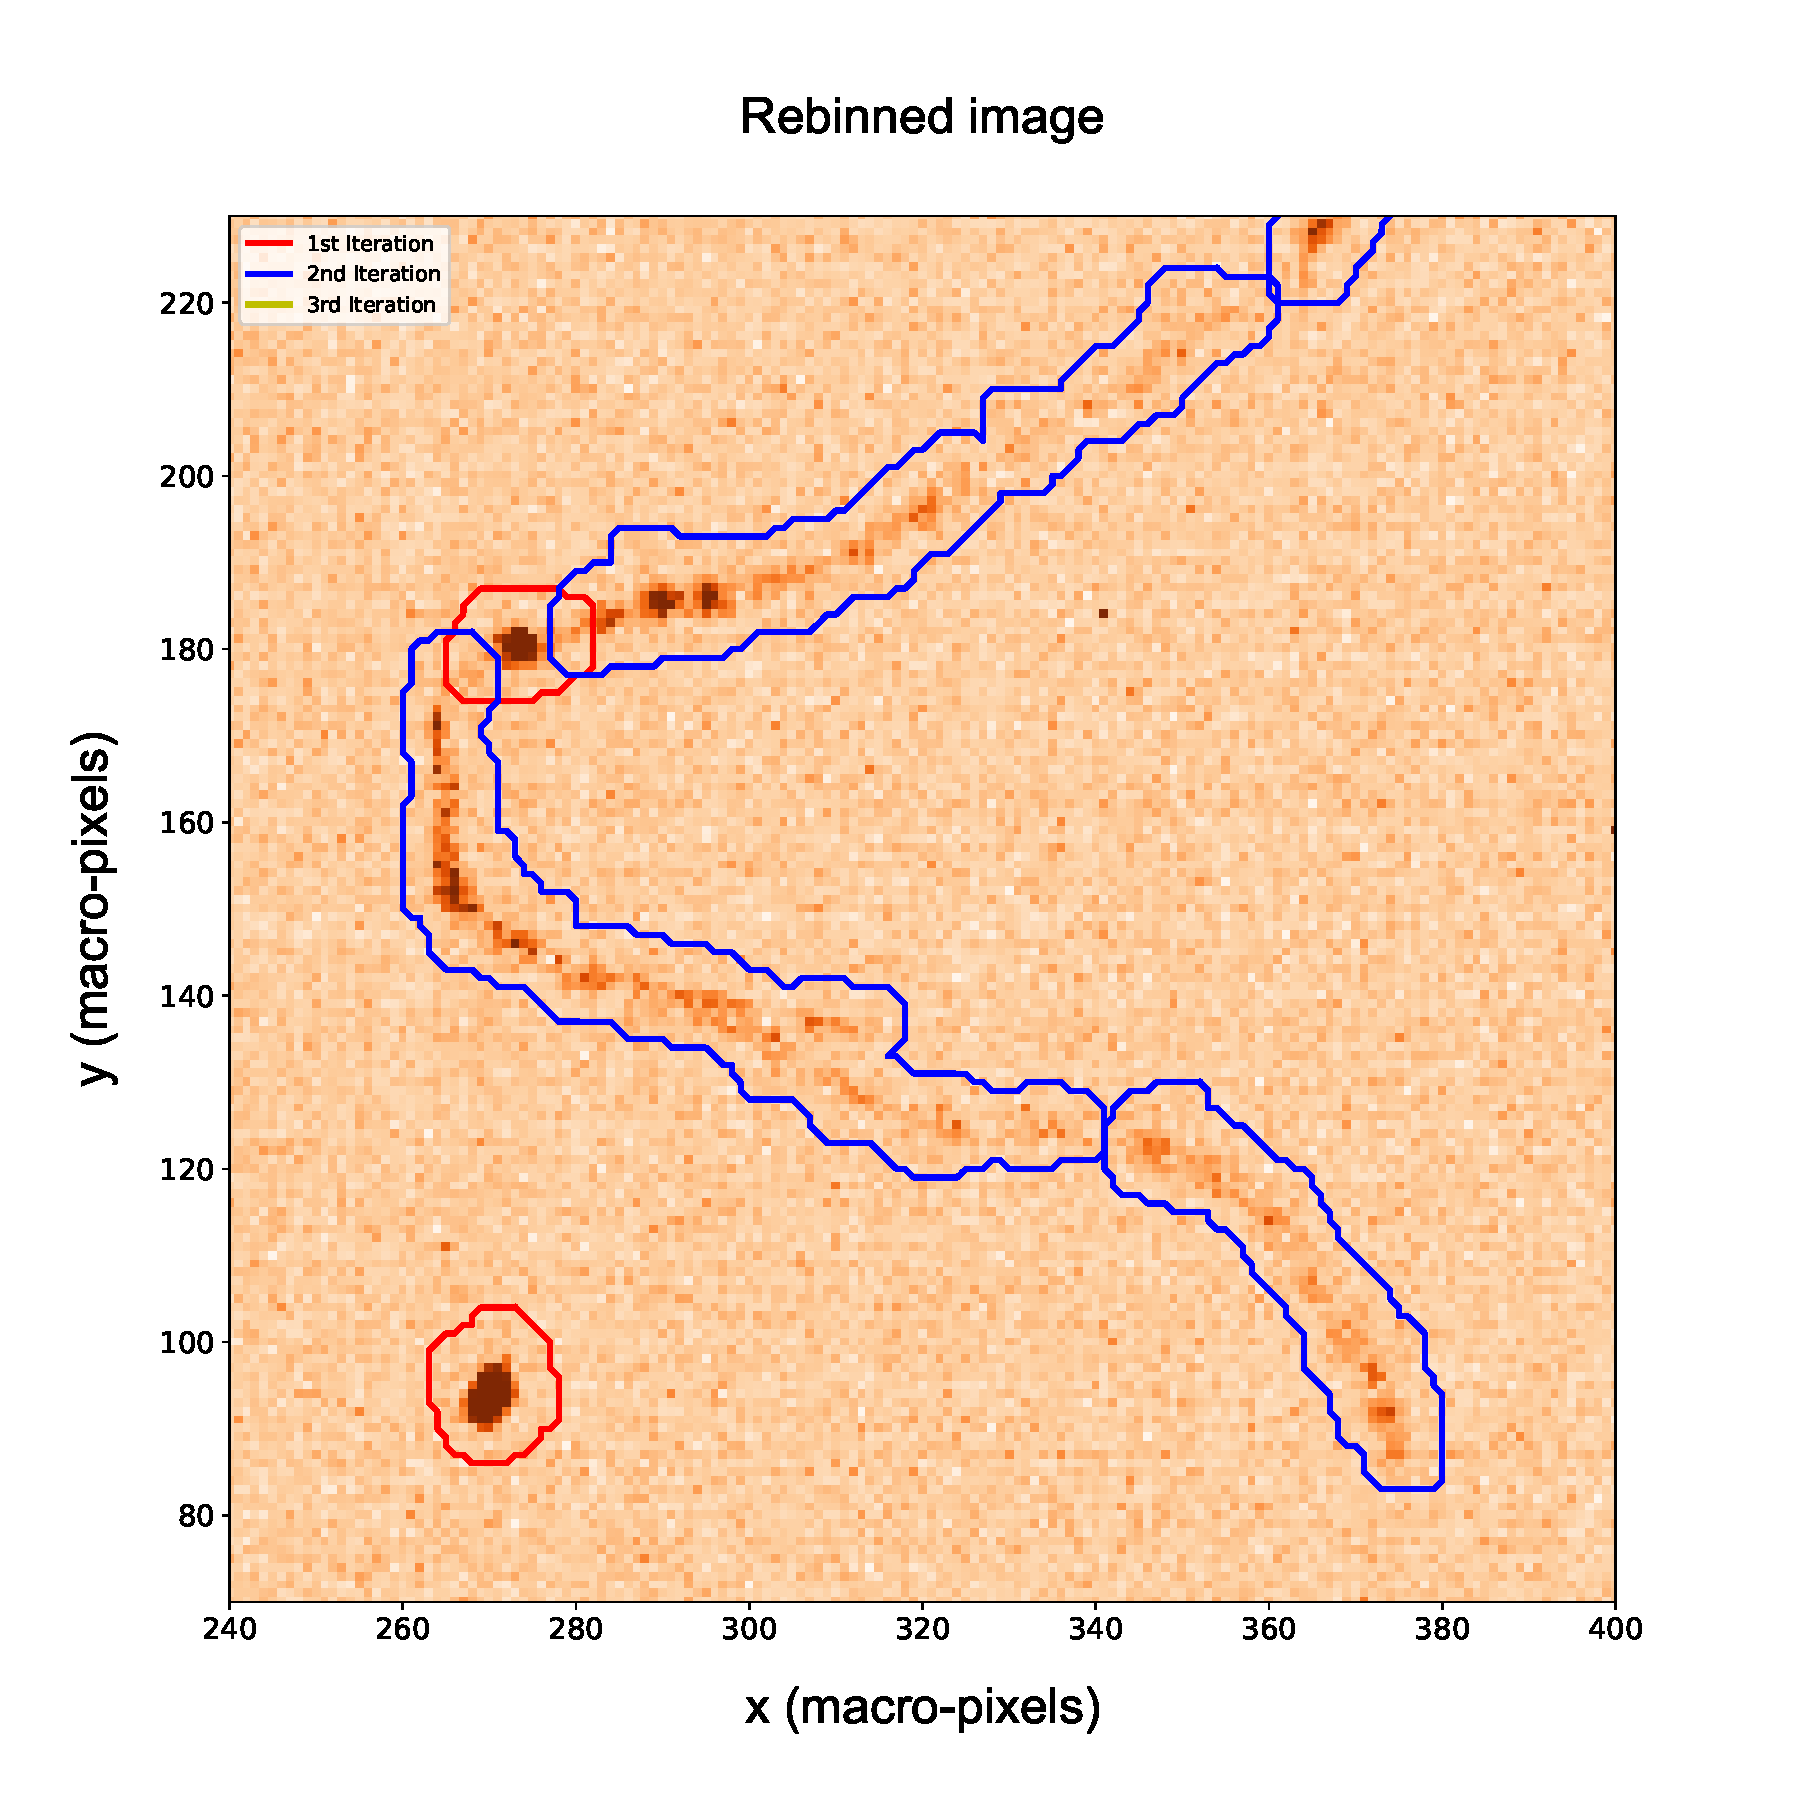
\includegraphics[width=0.49\linewidth]{figures/pic_run02317_ev8_all_3D_paper}

      \caption{Basic clusters reconstructed with the \idbscan
    algorithm in the low resolution (512$\times$512) image for two
    example events with very different patterns. Continuous lines
    represent the approximate contours of the reconstructed basic
    clusters of the first (red line) or second (blue line) \idbscan
    iteration. Left: clusters on spots from \fe source, two of which
    are merged together. Right: Track from natural radioactivity and a
    nuclear recoil candidate in an event with \ambe source. The long
    track is split in several basic clusters of different \idbscan
    iteration. \label{fig:basic_clusters}}

   \end{center}
\end{figure}
